\documentclass[../../main/main.tex]{subfiles}
\graphicspath{{./figures/}}

\dominitoc
\faketableofcontents

\makeatletter
\renewcommand{\@chapapp}{\'Electrocin\'etique -- chapitre}
\makeatother

% \toggletrue{student}
% \HideSolutionstrue
\toggletrue{corrige}
\renewcommand{\mycol}{black}
% \renewcommand{\mycol}{gray}

\begin{document}
\setcounter{chapter}{0}

\chapter{Circuits \'electriques dans l'ARQS}

\vfill

\begin{prgm}
	\begin{tcb}*(ror)"know"{Savoirs}
		\begin{itemize}[label=$\diamond$, leftmargin=10pt]
			\item Justifier que l’utilisation de grandeurs électriques
			      continues est compatible avec la quantification de la charge
			      électrique.
			\item Exprimer l’intensité du courant électrique en termes de débit de
			      charge.
			\item Exprimer la condition d’application de l’ARQS en fonction de la
			      taille du circuit et de la fréquence.
			\item Relier la loi des nœuds au postulat de la conservation de la charge.
			\item Citer les ordres de grandeur des intensités et des tensions dans
			      différents domaines d’application.
		\end{itemize}
	\end{tcb}

	\begin{tcb}*(ror)"how"{Savoir-faire}
		\begin{itemize}[label=$\diamond$, leftmargin=10pt]
			\item Utiliser la loi des mailles et la loi des nœuds
			\item Algébriser les grandeurs électriques et utiliser les conventions
			      récepteur et générateur.
		\end{itemize}
	\end{tcb}
\end{prgm}

\vfill
\minitoc
\vfill

\newpage
Pendant toute cette année nous nous plaçons dans un cadre particulier pour
l'étude de l'électrocinétique, celui de l'\textit{approximation des régimes
	quasi-stationnaires}, ou ARQS. Dans ce premier chapitre, nous nous attachons à
définir ce cadre et donnons les lois générales des circuits électriques que nous
pouvons alors établir.

\section{Courant électrique et intensité}
\subsection{Charge électrique}

\begin{tcb}[label=def:q, sidebyside](defi){Charge électrique}
	La charge électrique d'une particule, notée $q$, est une grandeur
	scalaire, caractérisant sa sensibilité aux interactions
	électromagnétiques.
	\tcblower
	\tcbsubtitle{\fatbox{Unités}}
	\psw{
		La charge électrique s'exprime en Coulomb, de symbole C.
	}
\end{tcb}
\begin{tcb}[label=exem:q](exem){Matière ordinaire}
	La matière ordinaire est constituée d'atomes, formés par~:
	\begin{itemize}[label=$\diamond$, leftmargin=10pt]
		\item \psw{
			      des \textbf{neutrons}, électriquement neutres (de charge nulle)~;
		      }
		\item \psw{
			      des \textbf{protons}, de charge positive et fondamentale~: $e =
				      \SI{1.6e-19}{C}$~;
		      }
		\item \psw{des \textbf{électrons}, de charge négative opposée à celle des
			      protons.}
	\end{itemize}
\end{tcb}
\begin{tcb}[label=prop:q](prop){Charge électrique et conservation}
	Un système électrique de charge totale $Q$ possède les propriétés
	suivantes~:
	\begin{enumerate}
		\item \psw{
			      $Q$ est \textbf{algébrique}~: elle peut être $\lessgtr 0$~;
		      }
		\item \psw{
			      $Q$ est \textbf{additive}~: $N$ particules de charges $q_{1, …,
						      N}$ forment une charge $Q = \sum_{i=1}^{N} q_i$~;
		      }
		\item \psw{
			      $Q$ est quantifiée~: $Q = k\times e$ avec $k \in \Zb$ et $e =
				      \SI{1.6e-19}{C}$~;
		      }
		\item \psw{
			      \fbox{Si le système est isolé, alors $Q$ est constante.}
		      }
	\end{enumerate}
\end{tcb}

\subsection{Courant électrique}
\begin{tcbraster}[raster columns=2, raster equal height=rows]
	\begin{tcb}[label=def:courant](defi){Courant électrique}
		Le courant électrique est un \textbf{mouvement d'ensemble} de particules
		chargées, appelées \textit{porteurs de charges}, dû à une action
		extérieure, le champ électrique $\Ef$.
	\end{tcb}
	\begin{tcb}[label=exem:porteurs](exem)'r'{Porteurs de charges}
		On étudiera deux types de porteurs~:
		\begin{enumerate}
			\item \psw{
				      Les \textbf{électrons libres} dans les conducteurs métalliques~;
			      }
			\item \psw{
				      Les \textbf{ions en solutions} dites électrolytiques.
			      }
		\end{enumerate}
	\end{tcb}
\end{tcbraster}

\subsection{Sens conventionnel du courant}

\begin{tcbraster}[raster columns=3, raster equal height=rows]
	\begin{tcolorbox}[blankest, raster multicolumn=2, valign=center]
		Les particules sont déplacées par un champ électrique $\Ef$ selon le sens
		algébrique de leur charge, avec une force $\Ff = q\Ef$ (voir mécanique
		première année)~: les charges avec $q>0$ sont déplacées dans le même sens
		que $\Ef$, celles de $q<0$ dans le sens opposé. Ils apportent cependant la
		\textit{même variation de charge} en valeur absolue. Avant de connaître
		quelles particules se déplaçaient dans les circuits électriques (les
		électrons), il a fallu choisir un sens conventionnel~:
	\end{tcolorbox}
	\begin{tcb}[label=def:sensconv](defi)'r'{Sens conventionnel}
		\psw{
			Le sens \textbf{conventionnel du courant} est le sens de déplacement des
			\textbf{porteurs charges positives} (réels ou hypothétiques). Les charges
			négatives se déplacent en sens contraire.
		}
	\end{tcb}
\end{tcbraster}

\subsection{Intensité du courant}

\begin{tcb}[label=def:intensité, sidebyside](defi){Intensité
			d'un courant}
	\psw{
		L'intensité électrique quantifie le \textbf{débit} de charges à travers une
		\underline{section orientée}, c'est-à-dire un \textbf{nombre de charges par
			unité de temps} dans la section étudiée. Une charge est comptée $+q$
		si elle traverse la section dans le même sens que son orientation (avec $q
			\lessgtr 0$), et $-q$ sinon.
	}
	\tcblower
	\tcbsubtitle{\fatbox{Unités}}
	\psw{
		L'intensité se mesure en ampère, de symbole A. De la définition, on a
		$\SI{1}{A} = \SI{1}{C.s^{-1}}$.
	}
	\tcbsubtitle{\fatbox{Notation}}
	Par convention, $i$ si elle varie, $I$ si elle est fixe.
\end{tcb}
\begin{tcb}[label=prop:intensité](prop){Expression de l'intensité}
	Soit un système électrique de \textbf{section orientée} $S$ traversée par
	des charges électriques. Si une quantité de charge $\delta q$ la traverse
	entre deux instants $t$ et $t + \delta t$, l'intensité $i$ du courant sera
	$i = \delta q/\delta t$, d'où en prenant la limite
	\psw{
		\[
			\boxed{
				i(t) =
				\lim_{\delta t \ra 0} \frac{\delta q}{\delta t} =
				\dv{q}{t}
			}
		\]
	}
	\vspace{-15pt}
\end{tcb}
\begin{tcb}[label=impl:intensconv](impl){Signe et sens réel}
	Si $i > 0$, alors $\de q > 0$~: pendant $\dd{t}$, il y a eu une traversée
	de charges avec résultante positive \textit{dans le sens orienté}. Comme le
	sens conventionnel est \textbf{celui des charges positives}, on retiendra
	\begin{itemize}
		\item si $i > 0$, le sens conventionnel est respecté~;
		\item si $i < 0$, le sens conventionnel est opposé à l'orientation
		      choisie.
	\end{itemize}
\end{tcb}
\begin{tcb}[label=nota:intensconv, sidebyside, righthand ratio=.4](nota){Représentation du sens}
	En représentant un fil électrique par un trait rectiligne, on oriente la
	section avec une flèche. La grandeur ainsi définie peut être $\lessgtr 0$.
	Si on la flèche dans l'autre sens, sa valeur est opposée.
	\tcblower
	\begin{center}
		\switch{
			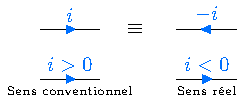
\includegraphics[width=\linewidth, draft=true]{intensconv}
		}{
			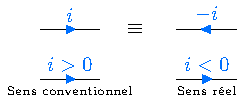
\includegraphics[width=\linewidth]{intensconv}
		}
	\end{center}
\end{tcb}
\begin{tcb}[label=impo:courantintensité](impo){Courant et intensité}
	Il vous faut savoir différencier le courant et l'intensité du courant~:
	\smallbreak
	\begin{isd}[cnt]
		\psw{
			Le courant est le \textit{phénomène physique}.
		}
		\vspace*{-10pt}
		\tcblower
		\psw{
			L'intensité est la \textit{quantification algébrique}.
		}
		\vspace*{-10pt}
	\end{isd}
\end{tcb}
\begin{tcb}[label=odgr:intensité](odgr){Intensités}
	Les valeurs mesurées sont~:
	\begin{itemize}[label=$\diamond$, leftmargin=10pt]
		\item $\approx \SI{1}{mA}$ pour l'électronique du quotidien
		      (téléphone)~;
		\item $\SIrange{1}{10}{A}$ pour l'électroménager (four,
		      aspirateur…)~;
		\item $\approx \SI{e2}{A}$ pour l'électrotechnique (TGV~:
		      $\SIrange{500}{1000}{A}$).
	\end{itemize}
	Le seuil létal pour le corps dépend de la durée de traversée, mais est
	\textbf{très faible}~: \SI{40}{mA} pendant 3 secondes, ou \SI{300}{mA}
	pendant \SI{0.1}{seconde}.
\end{tcb}
\begin{tcb}(appl){Exercice d'application}
	Un générateur délivre une intensité $I = \SI{3.0}{A}$. Quel est le
	nombre d'électrons émis chaque seconde~? Quelle durée faut-il à ce
	générateur pour émettre \num{1000} électrons~?
	\tcblower
	\psw{
		Par définition, $I = \Delta{Q}/\Delta{t}$, et $\Delta{Q} = Ne$ avec $N$ le
		nombre d'électrons et $e$ la charge élémentaire. Ainsi,
		\[
			\boxed{N = \frac{\Delta{Q}}{e} = \frac{I\Delta{t}}{e}}
			\qav
			\left\{
			\begin{array}{rcl}
				I         & = & \SI{3.0}{A}
				\\
				\Delta{t} & = & \SI{1}{s}
				\\
				e         & = & \SI{1.6e-19}{C}
			\end{array}
			\right.
			\qquad
			\mathrm{A.N.~:}\enskip
			\xul{
				N \approx \num{1.9e19}
			}
		\]
		On inverse la relation pour trouver
		\[
			\boxed{\Delta{t} = \frac{1000e}{I}}
			=
			\xul{\SI{5.3e-17}{s}}
		\]
	}
	\vspace*{-15pt}
\end{tcb}

\section{Tension et potentiel}
\subsection{Définition}
\begin{tcb}[label=def:tension, sidebyside](defi){Potentiel et tension}
	On appelle \textbf{potentiel} électrique la grandeur physique reliant la
	capacité d'un point à attirer les charges négatives~: plus le potentiel
	est élevé plus il les attire.
	\bigbreak
	On appelle \textbf{tension} ou \textbf{différence de potentiel} entre deux
	points la différence entre les valeurs du potentiel en chacun des points.
	\tcblower
	\tcbsubtitle{\fatbox{Unités}}
	\psw{
		Le potentiel, et par extension la différence de potentiel, s'exprime en
		Volt, de symbole V.
	}
	\tcbsubtitle{\fatbox{Notation}}
	$u$ si variable, $U$ sinon.
	\tcbsubtitle{\fatbox{En pratique}}
	\textbf{Seules les tensions se mesurent}.
\end{tcb}
\begin{tcb}[label=nota:tension, sidebyside, righthand ratio=.4](nota){Potentiel et tension}
	Il est convenu d'écrire le potentiel en un point A~: $V_A$, et la
	tension \textbf{entre les points} A et B~: $U_{AB} = V_A - V_B$. Sur un
	schéma, la tension est représentée par une flèche partant du
	\textbf{second potentiel vers le premier}.
	\tcblower
	\begin{center}
		\switch{
			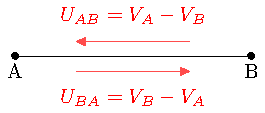
\includegraphics[width=\linewidth, draft=true]{tensionconv}
		}{
			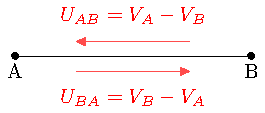
\includegraphics[width=\linewidth]{tensionconv}
		}
	\end{center}
\end{tcb}
\begin{tcb}[label=impl:tension](impl){Signe d'une tension}
	\begin{itemize}
		\item
		      \psw{
			      $U_{AB} > 0$ si $V_A > V_B$ et inversement~;
		      }
		\item
		      \psw{
			      \fbox{$U_{AB} = - U_{BA}$}~;
		      }
		\item
		      \psw{
			      \fbox{$U_{AB} = U_{AC} + U_{CB}$}.
		      }
	\end{itemize}
	\begin{center}
		\textbf{Attention} cependant, la flèche est opposée au sens usuel pour
		un vecteur $\overrightarrow{AB}$.
	\end{center}
\end{tcb}
\begin{tcb}[label=odgr:tensions](odgr){Tensions}
	Les valeurs mesurées sont~:
	\begin{itemize}
		\item $\approx \SIrange{0.100}{5}{V}$ pour l'électronique du
		      quotidien (téléphone)~;
		\item $\approx \SI{220}{V}$ pour l'électroménager (four,
		      aspirateur…)~;
		\item $\approx \SIrange{100}{1000}{kV}$ pour l'électrotechnique
		      (lignes hautes tensions).
	\end{itemize}
\end{tcb}

\subsection{Référence du potentiel~: la masse}

\begin{tcb}[label=def:masse, sidebyside](defi){Masse d'un circuit}
	\psw{
		L'origine des potentiels d'un circuit est appelée la \textbf{masse} du
		circuit. C'est le point où $V = 0$. Elle sert de référence et est
		choisie arbitrairement, les tensions pouvant être négatives, et permet
		la mesure des tensions.
	}
	\vspace{-15pt}
	\tcblower
	Dans un circuit électrique, elle est représentée par l'un de ces deux
	symboles
	\begin{center}
		\switch{
			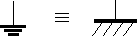
\includegraphics[width=\linewidth, draft=true]{masse}
		}{
			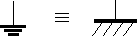
\includegraphics[width=\linewidth]{masse}
		}
	\end{center}
\end{tcb}

\section{Analogie électro-hydraulique}

Les phénomènes régissant la tension et le courant électrique sont en tous points
semblables à ceux régissant le dénivelé et le courant dans un circuit
hydraulique. Cette vision permet de mieux comprendre le vocabulaire employé.

Considérons une analogie hydraulique~: dans une conduite d'eau horizontale entre
deux récipients, l'eau ne s'écoulera pas. Un courant d'eau apparaîtra si on
surélève l'un des récipients par rapport à l'autre, et ce courant sera
\textbf{vers le plus bas}. Le récipient surélevé va finir par se vider et le
courant d'eau cessera. C'est la \textbf{différence d'altitude} entre les deux
récipients qui permet la \textbf{circulation du courant}. Les deux sens ne sont
pas équivalents, le courant d'eau ne se produit spontanément que vers le bas.

Par analogie avec l'\textbf{altitude} $h$ de la canalisation, on définit le
\textbf{potentiel} électrique $V$. Ainsi, un courant électrique apparaît
spontanément dans le sens des \textbf{potentiels décroissants}. Pour que le
courant remonte les potentiels, il faut « pomper » les charges à l'aide d'un
générateur. L'équivalent électrique du dénivelé (différence d'altitudes) en
hydraulique est la tension (différence de potentiels). Voir ce site et
l'animation flash~: \href{https://www.pccl.fr/physique\_chimie\_college\_lycee/quatrieme/electricite/analogie\_hydraulique.htm}
{https://www.pccl.fr/physique\_chimie\_college\_lycee/quatrieme/electricite/}

\begin{figure}[h]
	\centering
	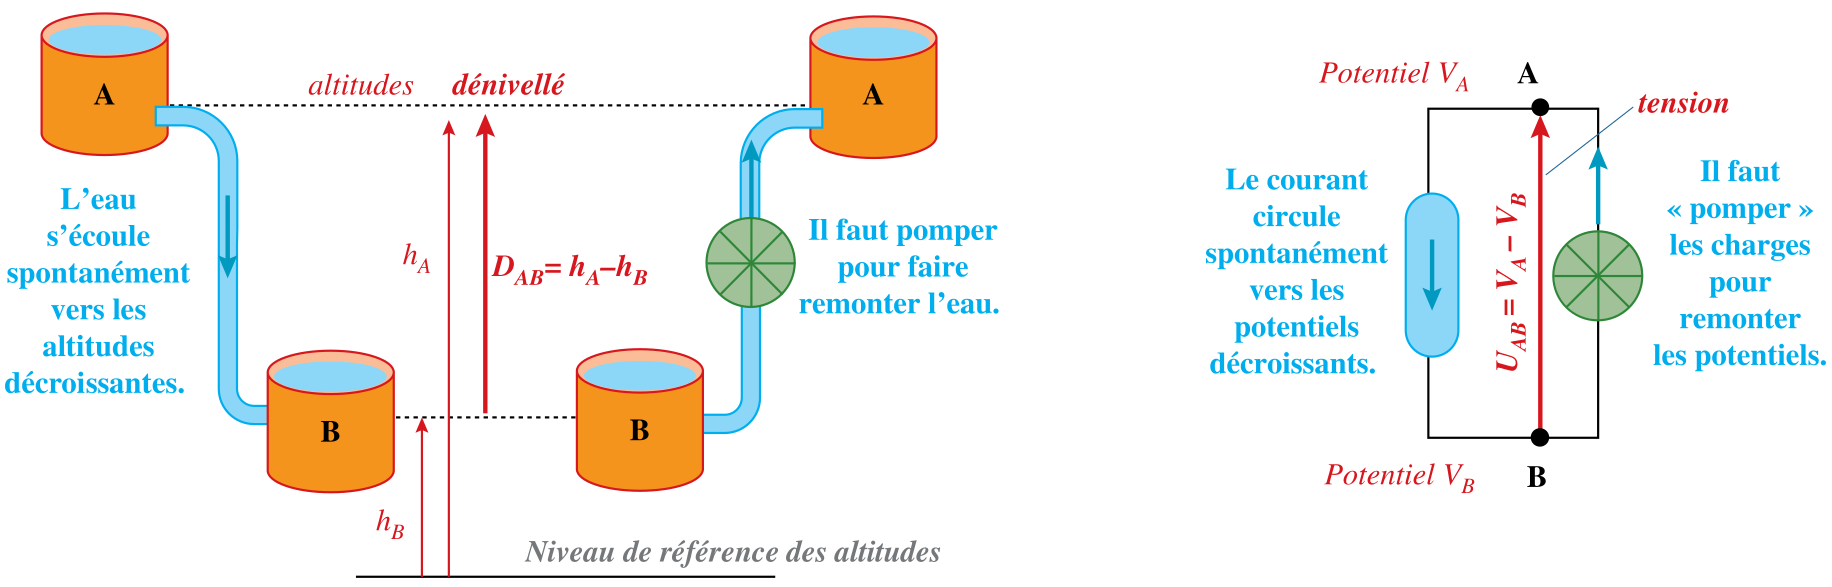
\includegraphics[width=\linewidth]{anal_elec-hydro.png}
	\label{fig:anal_elec-hydro}
\end{figure}

On définit de la même manière la puissance~: pour l'hydraulique, la puissance
d'un courant est égal au produit du dénivelé et du débit, en
électrocinétique on aura donc
\[\boxed{\left| P \right| = U\cdot I}\]
Nous discutons de son signe dans la section suivante.

\section{Vocabulaire des circuits électriques}
\subsection{La base}
\begin{tcb}[label=def:circuits, tabularx={Y|Y|Y}](defi){Base}
	\tcbsubtitle{\fatbox{Circuit électrique}}
	Ensemble de composants électriques reliés entre eux par des fils
	métalliques conducteurs. &
	\tcbsubtitle{\fatbox{Schéma électrique}}
	Représentation simplifiée d'un circuit dans laquelle les composants sont
	représentés par des symboles standardisés et les fils les reliant par des
	traits. &
	\tcbsubtitle{\fatbox{Dipôle}}
	Composant électriques comportant deux bornes sur lesquelles sont branchés
	des fils conducteurs.
\end{tcb}
\begin{tcb}[label=exem:circuits, sidebyside](exem){Circuit et schéma}
	\begin{center}
		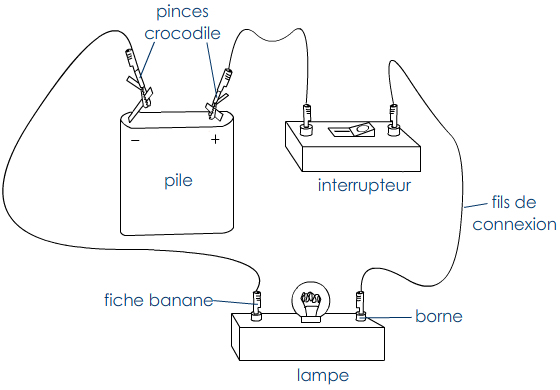
\includegraphics[width=.7\linewidth]{circuit_simple_dessin.jpg}
	\end{center}
	\tcblower
	\begin{center}
		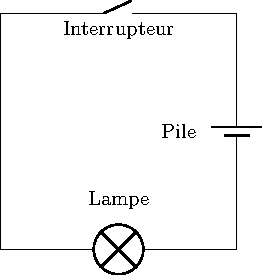
\includegraphics[width=.5\linewidth]{circuit_simple.pdf}
	\end{center}
\end{tcb}

\subsection{Décrire un circuit}
\begin{tcb}[label=def:descri, sidebyside, righthand ratio=.4](defi){Description}
	\begin{itemize}[leftmargin=50pt]
		\item[\textbf{Nœud}]: \psw{
			      point où se rejoignent au moins 3 fils.
		      }
		\item[\textbf{Branche}]: \psw{
			      portion du circuit entre deux nœuds voisins.
		      }
		\item[\textbf{Maille}]: \psw{
			      succession de branches partant et retournant au même point.
		      }
	\end{itemize}
	\tcblower
	\begin{center}
		\switch{
			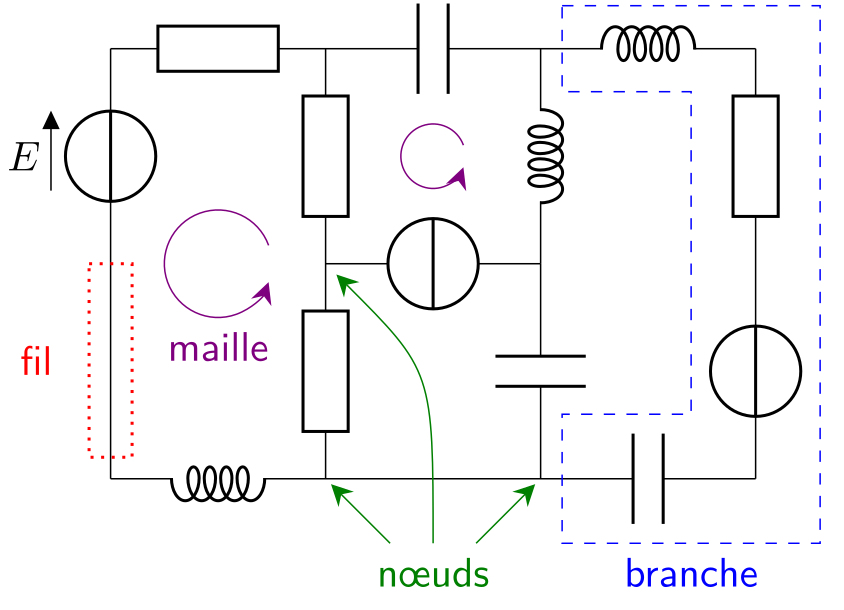
\includegraphics[width=\linewidth, draft=true]{circuit_voca}
		}{
			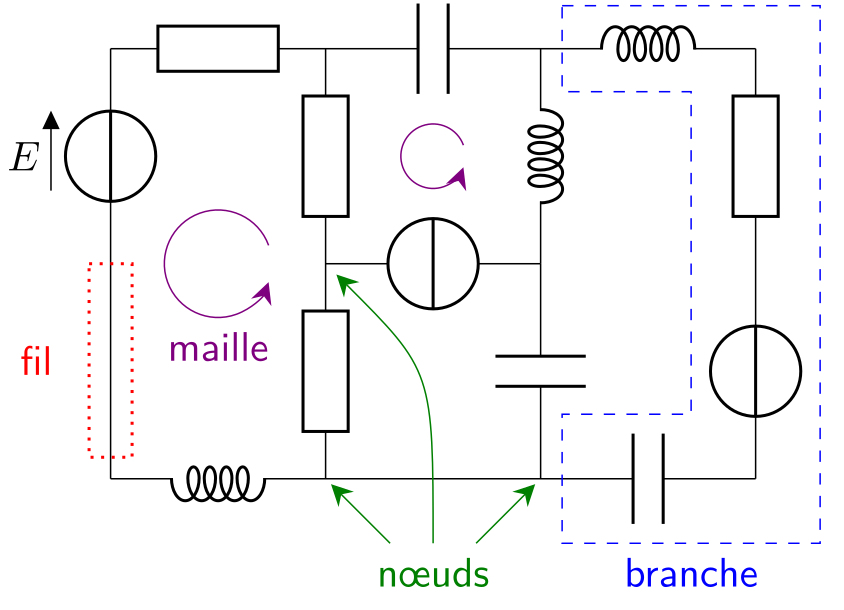
\includegraphics[width=\linewidth]{circuit_voca}
		}
	\end{center}
\end{tcb}

\subsection{Conventions générateur et récepteur}
Chacune des orientations de l'intensité et de la tension est arbitraire. Pour
étudier le comportement d'un dipôle, il nous faut choisir une dernière
convention donnant l'orientation relative de la tension $u$ à ses bornes et de
l'intensité $i$ du courant la traversant. Celle-ci dépend de la nature
génératrice ou réceptrice d'un dipôle afin de respecter leurs physiques
respectives.

\begin{tcb}[label=def:convrg, sidebyside, righthand width=.3\linewidth](defi)
	{Conventions récepteur et générateur}
	En convention \textbf{récepteur}, l'intensité $i$ traversant un dipôle et la
	tension $u$ à ses bornes sont orientées en \textbf{sens contraires}.
	\bigbreak
	En convention \textbf{générateur}, l'intensité $i$ traversant un dipôle et la
	tension $u$ à ses bornes sont orientées en \textbf{dans le même sens}.
	\tcblower
	\begin{center}
		\switch{
			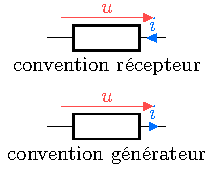
\includegraphics[width=\linewidth, draft=true]{rgconv}
		}{
			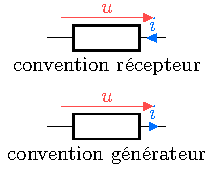
\includegraphics[width=\linewidth]{rgconv}
		}
	\end{center}
\end{tcb}

\subsection{Relation entre dipôles}
\begin{tcb}[sidebyside, righthand ratio=.4](defi){Série}
	Deux dipôles sont dits \textbf{en série} s'ils partagent \textbf{une et une
		seule borne} qui \textbf{n'est pas un nœud} (de laquelle ne part aucune
	autre branche).
	\tcblower
	\begin{center}
		\switch{
			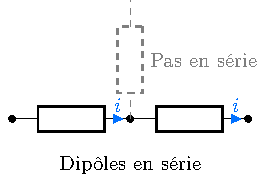
\includegraphics[width=\linewidth, draft=true]{serie}
		}{
			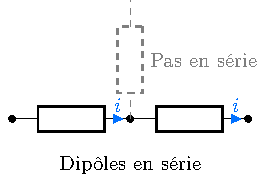
\includegraphics[width=\linewidth]{serie}
		}
	\end{center}
\end{tcb}
\begin{tcb}[label=ror:serdiv, fontupper=\Large, cnt](ror){Série}
	Deux dipôles \textbf{en série} sont traversés par la \textbf{même
		intensité}.
\end{tcb}

\begin{tcb}[sidebyside, righthand ratio=.4](defi){Dérivation}
	Deux dipôles sont dits \textbf{en dérivation/en parallèle} s'ils partagent
	leurs \textbf{deux bornes}.
	\tcblower
	\begin{center}
		\switch{
			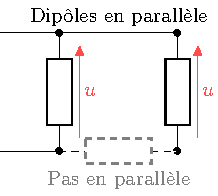
\includegraphics[width=\linewidth, draft=true]{derivation}
		}{
			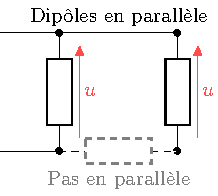
\includegraphics[width=\linewidth]{derivation}
		}
	\end{center}
\end{tcb}
\begin{tcb}[label=ror:serdiv, fontupper=\Large, cnt](ror){Dérivation}
	Deux dipôles \textbf{en parallèle/dérivation} ont la \textbf{même tension} à
	leurs bornes.
\end{tcb}

\begin{tcb}[label=rema:serdiv, halign=center](rema){Série et dérivation}
	\textbf{Deux dipôles peuvent n'être ni en série, ni en dérivation.}
\end{tcb}
\begin{tcb}[label=exer:serdiv](appl){Exercice d'application}
	\begin{minipage}{0.65\linewidth}
		Pour le schéma ci-dessous, indiquer si les couples de dipôles suivants
		sont en série, en parallèle ou ni l'un ni l'autre~: ($R_1$ et $R_0$) ;
		($r_0$ et $r_2$) ; ($R_2$ et $R_0$) ; ($R_3$ et $R_2$).
	\end{minipage}
	\begin{minipage}{0.35\linewidth}
		\begin{center}
			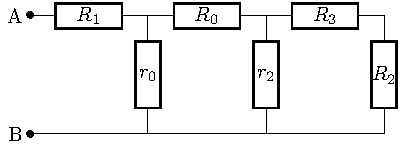
\includegraphics[width=\linewidth]{exer_serdiv}
		\end{center}
	\end{minipage}
	\tcblower
	\psw{
		($R_1$ et $R_0$)~: rien. ($r_0$ et $r_2$)~: rien. ($R_2$ et $R_0$)~: rien.
		($R_3$ et $R_2$)~: série.
	}
\end{tcb}

\subsection{Mesures de tensions et d'intensités}

\begin{tcb}[label=prop:mesure, sidebyside, righthand ratio=.4](prop){Voltmètre et ampèremètre}
	Une \textbf{tension} se mesure à l'aide d'un \textbf{voltmètre}.
	\smallbreak
	Un voltmètre se monte en \textbf{parallèle}.
	\smallbreak
	Pour mesurer la tension $U_{AB}$ il faut placer la borne COM au point B.

	\bigbreak

	Une \textbf{intensité} se mesure à l'aide d'un \textbf{ampèremètre}.
	\smallbreak
	Un ampèremètre se monte en \textbf{série}.
	\smallbreak
	Le sens du courant affiché par l'ampèremètre est relié au sens de branchement.
	\tcblower
	\begin{center}
		\switch{
			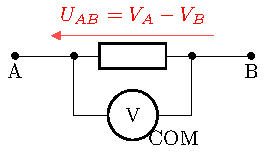
\includegraphics[width=\linewidth, draft=true]{voltmetre}
		}{
			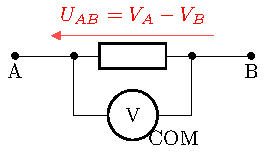
\includegraphics[width=\linewidth]{voltmetre}
		}
	\end{center}
	\begin{center}
		\switch{
			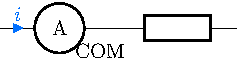
\includegraphics[width=\linewidth, draft=true]{amperemetre}
		}{
			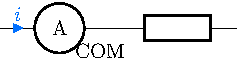
\includegraphics[width=\linewidth]{amperemetre}
		}
	\end{center}
\end{tcb}

\section{Lois fondamentales des circuits électriques dans l'ARQS}

\subsection{L'approximation des régimes quasi-stationnaires (ARQS)}

\sde[right](loi){ARQS}{
	\psw{
		L'approximation des régimes quasi-stationnaires correspond à considérer
		que les variations des grandeurs électriques se propagent
		\textit{instantanément} dans la totalité d'un circuit. Si sa longueur
		totale est $L$ et si la fréquence de variation du signal électrique est
		$f$ (ou temps de variation $T$), l'ARQS est applicable si
	}
}{
	\psw{
		$
			\begin{gathered}
				L \ll \frac{c}{f}
				\Longleftrightarrow
				\boxed{L \ll cT}
				\Longleftrightarrow T \gg \frac{L}{c}
			\end{gathered}
		$
	}
}
\begin{tcb}[label=demo:arqs](demo){ARQS}
	\psw{
		Dans un fil, les électrons sont mis en mouvement par un champ
		électrique. La théorie électromagnétique nous montre que le champ
		électrique est une onde qui se déplace à la célérité $c \approx
			\SI{3.00e8}{m.s^{-1}}$. Ainsi, la variation du potentiel dans un fil se
		fait à vitesse finie et il y a en général un \textbf{retard à la
			propagation}. Si le champ varie dans le temps avec une période $T$, il
		varie dans l'espace avec une période $\lambda = cT$. On peut alors
		considérer que le champ électrique est le même le long d'un fil si sa
		taille est beaucoup plus petite que la longueur d'onde $\lambda$.
	}
\end{tcb}
\begin{tcb}(appl){Application}
	Vérifier si l'ARQS est valable pour les 3 cas suivants~:
	\begin{itemize}
		\item En travaux pratiques avec $f = \SI{1}{kHz}$~;
		\item Sur une ligne à haute tension de \SI{100}{km} à basse fréquence
		      (\SI{50}{Hz})~;
		\item À l'intérieur d'une carte mère d'un ordinateur de \SI{10}{cm} à
		      $f \approx \SI{1}{GHz}$.
	\end{itemize}
	\tcblower
	\psw{
		Oui, si $L \ll \SI{300}{km}$~; oui, si $L \ll \SI{6000}{km}$~; non, $Lf =
			\SI{1e8}{m.s^{-1}} \neg\ll c$.
	}
\end{tcb}
\begin{tcb}[label=def:regimecontvar, sidebyside](defi){Régimes continu et variable}
	\tcbsubtitle{\fatbox{Régime continu}}
	Toutes les intensités et les tensions du circuit
	sont constantes ou cours du temps.
	\tcblower
	\tcbsubtitle{\fatbox{Régime variable}}
	Au moins une tension ou une intensité du circuit
	varie au cours du temps.
\end{tcb}

\subsection{Loi des nœuds}

Dans le cadre de l'ARQS, il ne peut y avoir d'accumulation de charges en un
point du circuit~: toutes les charges apportées par un courant doivent
immédiatement être évacuées par un autre courant, donnant lieu aux lois des
branches et des nœuds~:
\begin{tcb}[label=loi:branche, sidebyside, halign upper=center](loi){Loi des branches}
	\textbf{L'intensité est la même le long d'une branche}.
	\tcblower
	\begin{center}
		\switch{
			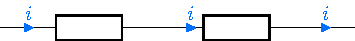
\includegraphics[width=\linewidth, draft=true]{ldb}
		}{
			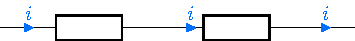
\includegraphics[width=\linewidth]{ldb}
		}
	\end{center}
\end{tcb}
\begin{tcb}[label=loi:noeud, sidebyside, halign upper=center](loi){Loi des nœuds}
	\textbf{La somme des intensités dirigées vers un nœud est égale à la somme de
		celles dirigées à l'opposé}, ou \textbf{la somme algébrique des intensités
		en un point est nulle}.
	\tcblower
	\begin{center}
		\switch{
			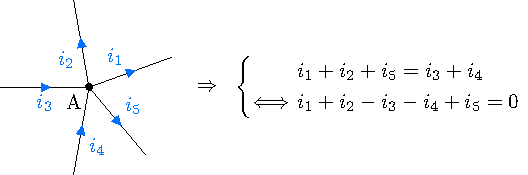
\includegraphics[width=\linewidth, draft=true]{ldn}
		}{
			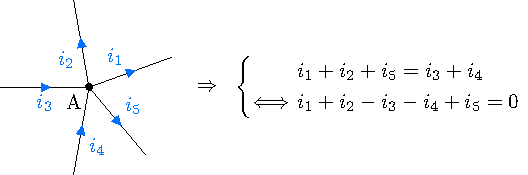
\includegraphics[width=\linewidth]{ldn}
		}
	\end{center}
\end{tcb}

\subsection{Loi des mailles}

Avec le principe d'additivité des tensions, on en déduit la loi des mailles.
\begin{tcb}[label=loi:mailles, sidebyside, halign upper=center](loi){Loi des mailles}

	\textbf{Dans une maille orientée, la somme algébrique des tensions est nulle
	}, ou \textbf{la somme des tensions dans le sens de la maille est égale à la
		somme des tensions dans le sens opposé}
	\tcblower
	\begin{center}
		\switch{
			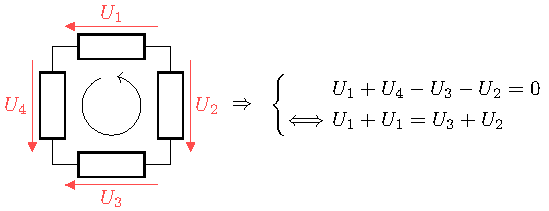
\includegraphics[width=\linewidth, draft=true]{ldm}
		}{
			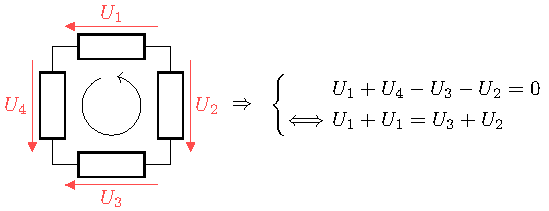
\includegraphics[width=\linewidth]{ldm}
		}
	\end{center}
\end{tcb}

\begin{tcb}[breakable](appl){Exercice d'application}
	\begin{minipage}{0.30\linewidth}
		Pour le circuit ci-contre, établir les liens entre les différents
		courants et les différentes tensions.
	\end{minipage}
	\begin{minipage}{0.70\linewidth}
		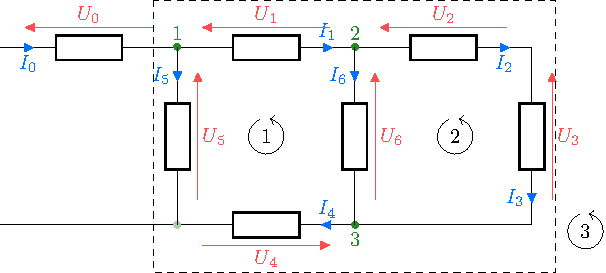
\includegraphics[width=\linewidth]{exer_ldnm}
	\end{minipage}
	\tcblower
	\begin{isd}[sidebyside align=top]
		\tcbsubtitle{\fatbox{Lois des nœuds}}
		\psw{
			\begin{itemize}
				\item $I_2 = I_3$ par unicité à droite ;
				\item $I_0 = I_1 + I_5$ par LdN 1 ;
				\item $I_1 = I_2 + I_6$ par LdN 2 ;
				\item $I_3 + I_6 = I_4$ par LdN 3.
			\end{itemize}
			Le dernier nœud, non numéroté, donne une relation redondante avec les
			autres.
		}
		\tcblower
		\tcbsubtitle{\fatbox{Lois des mailles}}
		\psw{
			\begin{itemize}
				\item $U_4 + U_6 + U_1 = U_5$ par LdM 1 ;
				\item $U_3 + U_2 = U_6$ par LdM 2 ;
			\end{itemize}
			La LdM 3 donne une relation redondante avec les deux premières : $U_4
				+ U_2 + U_3 + U_1 = U_5$ est la somme des deux.
		}
	\end{isd}
\end{tcb}

\subsection{Puissance électrocinétique}

\begin{tcb}[label=def:puissance, sidebyside, sidebyside align=top](defi){Puissance récepteur, générateur}
	\tcbsubtitle{\fatbox{Récepteur}}
	\psw{
		Un dipôle \textbf{fonctionne comme récepteur} s'il \textbf{reçoit de
			l'énergie} du reste système. Dans ce cas-là, sa puissance \textit{en
			convention récepteur} est $P_{\text{reçue}} = u\times i > 0$. Si après
		calcul une puissance reçue est négative, c'est que le dipôle est en fait
		générateur.
	}
	\tcblower
	\tcbsubtitle{\fatbox{Générateur}}
	\psw{
		Un dipôle \textbf{fonctionne comme générateur} s'il \textbf{fournit de
			l'énergie} au reste système. Dans ce cas-là, sa puissance \textit{en
			convention générateur} est $P_{\rm fournie} = u\times i > 0$. Si après
		calcul une puissance fournie est négative, c'est que le dipôle est en fait
		récepteur.
	}
\end{tcb}

\begin{tcb}[label=impo:convrg](impo){Puissances}
	\begin{tabularx}{\linewidth}{|Y*{2}{|Y}|}\hline
		                                                     &
		Dipôle \textcolor{ForestGreen}{récepteur}            &
		Dipôle \textcolor{CornflowerBlue}{générateur}
		\\\hline
		Convention récepteur
		\smallbreak $\textcolor{orange}{P_{\text{reçue}}}$   &
		\switch{
			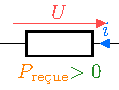
\includegraphics[width=3cm, draft=true]{rconvr}
		}{
			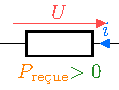
\includegraphics[width=3cm]{rconvr}
		}
		                                                     &
		\switch{
			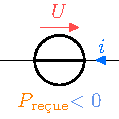
\includegraphics[width=3cm, draft=true]{gconvr}
		}{
			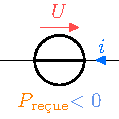
\includegraphics[width=3cm]{gconvr}
		}
		\\\hline
		Convention générateur
		\smallbreak $\textcolor{Purple}{P_{\text{fournie}}}$ &
		\switch{
			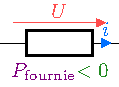
\includegraphics[width=3cm, draft=true]{rconvg}
		}{
			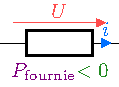
\includegraphics[width=3cm]{rconvg}
		}
		                                                     &
		\switch{
			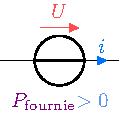
\includegraphics[width=3cm, draft=true]{gconvg}
		}{
			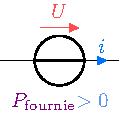
\includegraphics[width=3cm]{gconvg}
		}
		\\\hline
	\end{tabularx}
\end{tcb}

\begin{tcb}[label=prop:puiss](prop){Conservation de l'énergie}
	\psw{
		L'\textbf{énergie} est une \textbf{grandeur conservative}. Elle ne peut être
		crée ou détruite. Elle ne peut qu'être convertie d'une forme en une autre
		et/ou transférée d'un système à un autre. Il en découle que dans une maille,
		\textbf{les puissances reçues sont égales aux puissances émises},
		c'est-à-dire
		\[
			\boxed{\sum P_{\rm fournies} = \sum P_{\text{reçues}}}
		\]
	}
\end{tcb}

\end{document}
